\chapter{Testing}

The implementation described in the previous chapter now has to be tested.
The testing should show if the implemented system produces the required output.
Testing of single parts of the system like the interface from the application to the GPS receiver or the calculation of satellite positions is not the focus here.
The tests described are on the level of the whole system.
Multiple accuracy tests were planned to test different factors that could impact the system.
Most tests were planned to determine how accurate the DGPS system is compared to standard GPS.
Also the influences of the extreme conditiond on a sounding rocket should be determined with these tests as far as possible.
Unfortunately, there was not enough time to conduct all planned tests.
Only static accuracy tests were conducted.
The most representative is described in section \ref{sec:static_accuracy}.


\section{Testing Setup}

The setup to test the system does not differ much from the system described in the implementation chapter.
The difference is that for static accuracy tests, no wireless communication is needed.
The corrections can be sent directy to a second receiver plugged into the laptop which runs the application.
Two receivers are needed for the DGPS, one as reference station and one as user.
Additionally, a receiver has to measure the position without applying the corrections to have a reference to compare the DGPS to.
This setup can be achieved with only two receivers, when the postition output of the reference receiver is used as the uncorrected GPS measurement.

Needed to evaluate the tests are the position estimations with and without applying the corrections, and the PRCs.
The M8T receiver has the ability to log all its output.
It can later be retrieved with the u-blox software u-center.
The logging of the PRCs can be enabled in the DGPS Message Generator application.

Before the logged data can be evaluated, the messages have to be extracted from the bit straem.
A NMEA parser was written in C++ to extact the GxGGA messages and save them to a .csv file.
They contain GPS fix data like UTC time, latitude, longitude and altitude.
The evaluation is done with Matlab scripts that understands the format of the generated .csv files (Appendix \ref{appendix:matlab_code}).

\section{Static Accuracy}\label{sec:static_accuracy}

Static accuracy test means that the user receiver does not move and is at the same position as the reference station.
This test was done at a surveyed location to be able to measure the absolute position error.
The Swiss Federal Office of Topography Swisstopo manages the control points data used for natonal surveying.
Swisstopo makes the data available online in form of a map \cite{Swisstopo}.
The choosen test location is a control point on the Sonnenberg in Kriens.
Its exact position is given in the corresponding file (Appendix \ref{appendix:control_point_sonnenberg}).

\newpage

\subsection{Setup}

The reference coordinates are given in the local swiss reference frame LV95.
They have to be converted to the WGS84 reference frame in ECEF form.
This was done using the REFRAME online tool from Swisstopo.

\begin{figure}[ht]
 \centering
 \includegraphics[width=\textwidth]{images/measurement_kriens_setup.png}
 \caption{Measurement setup on the Sonnenberg in Kriens}
 \label{fig:measurement_kriens_setup}
\end{figure}

The measurement was conducted on the 26. Mai 2018 from 15:15 until 16:15.
The location can be seen in figure \ref{fig:measurement_kriens_setup}.
The control point is marked by a triangle on the manhole cover.
The two antennas were placed about 10 cm apart and 1 meter above the control point.

\newpage

\begin{figure}[ht]
 \centering
 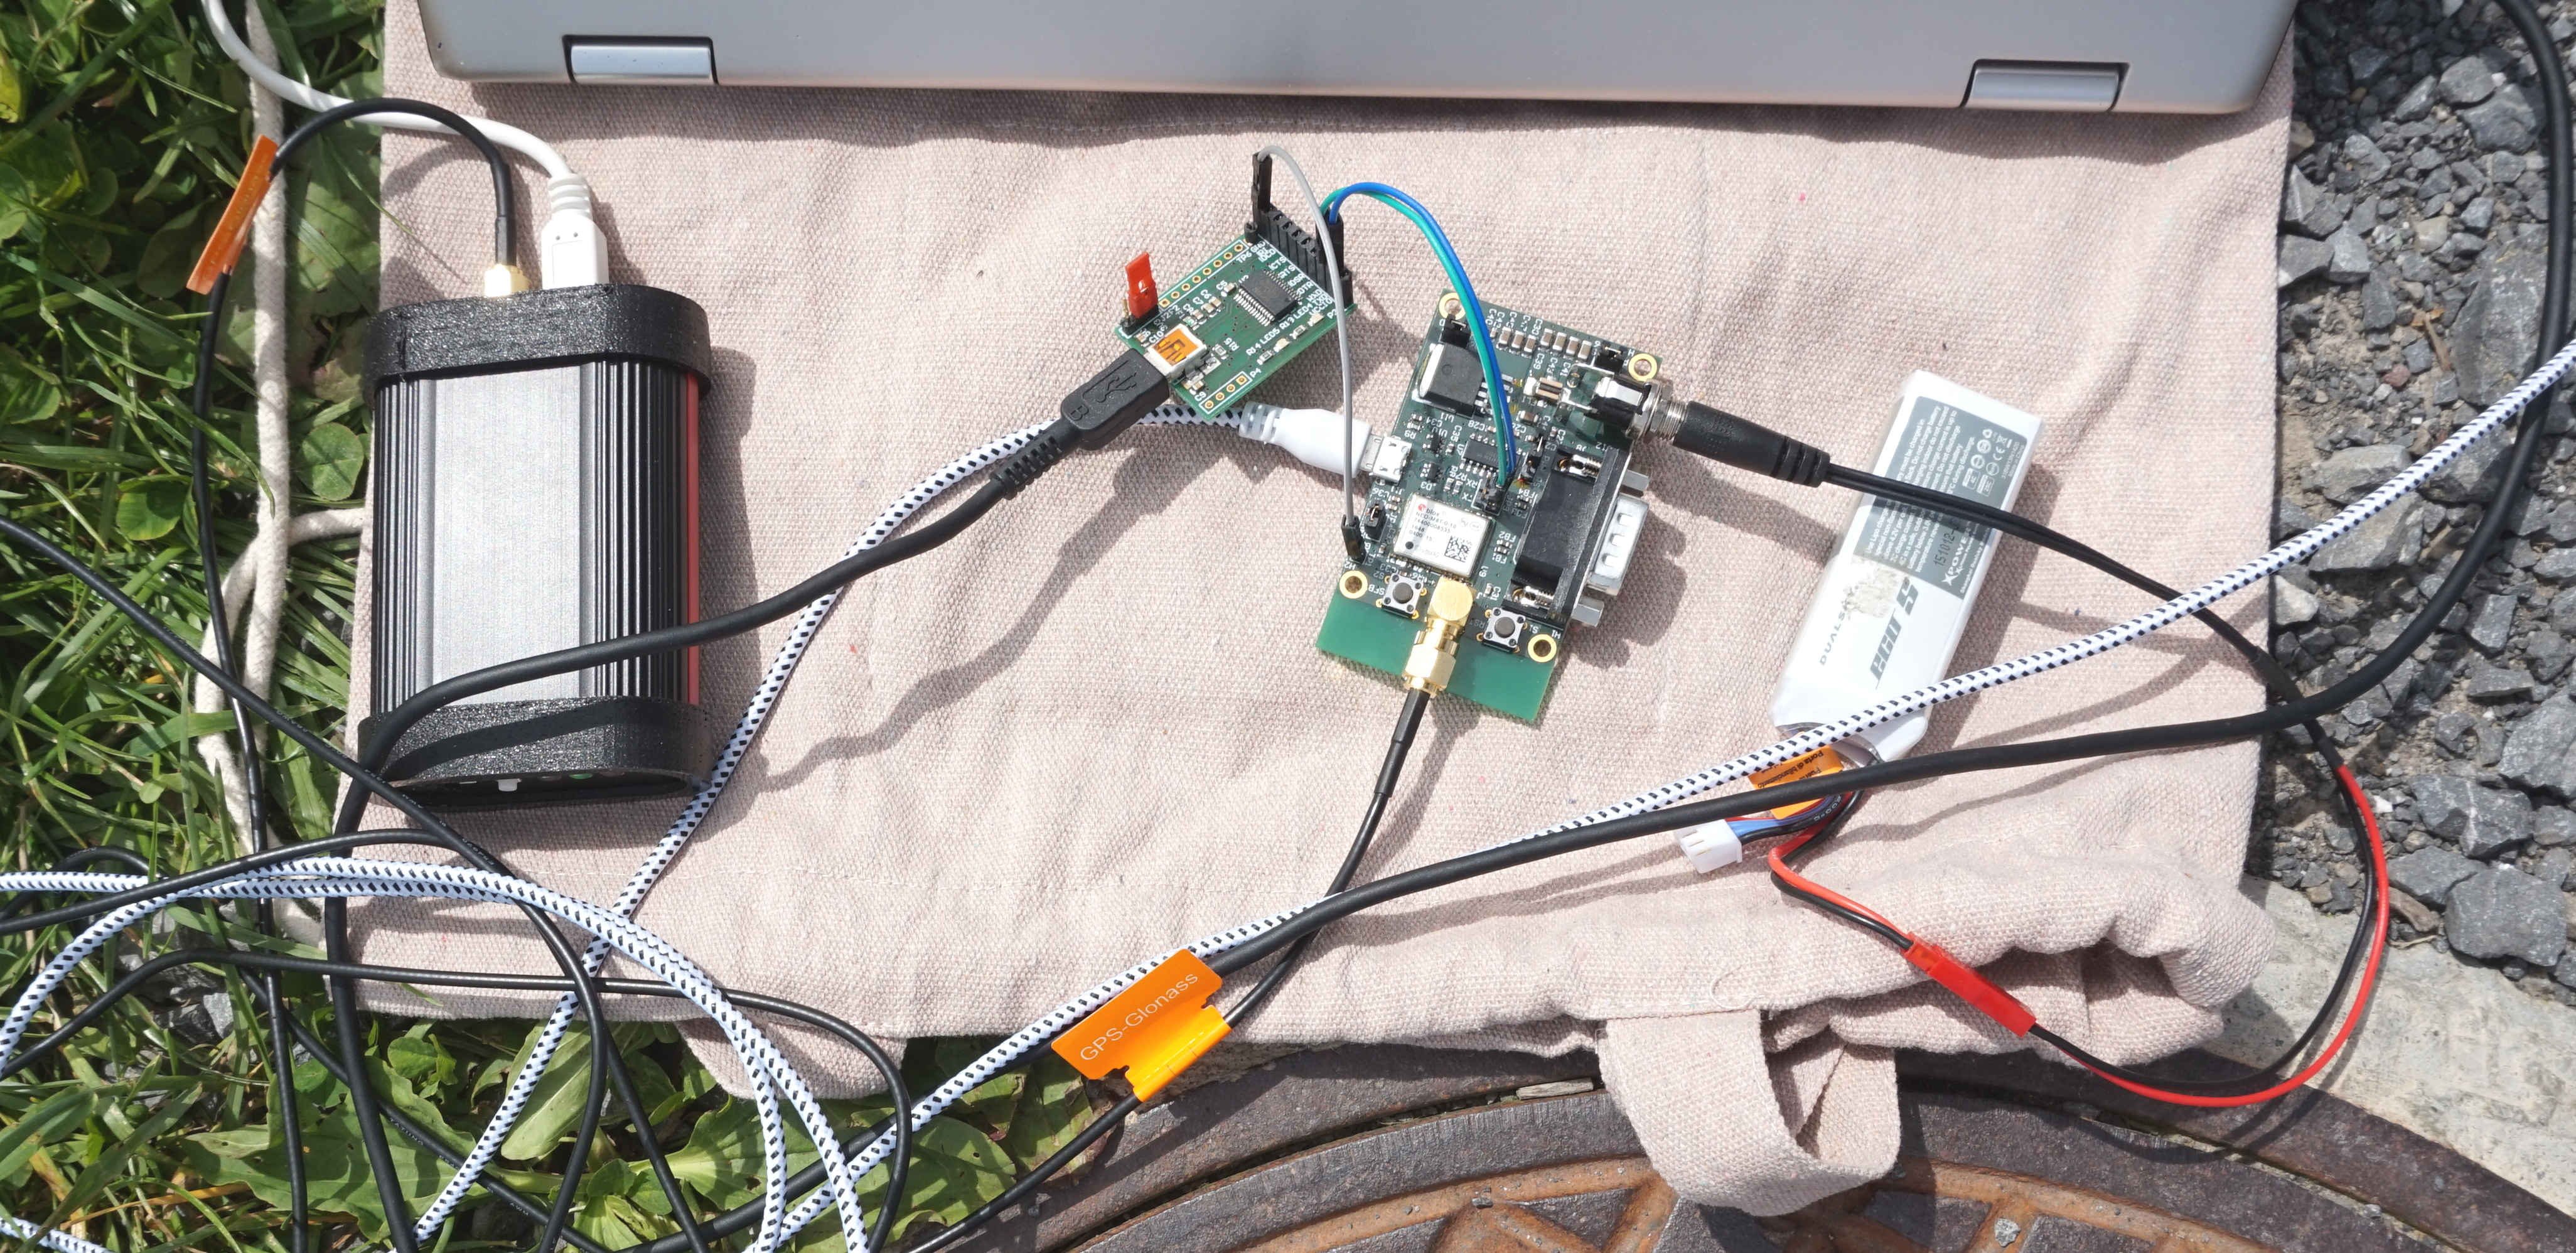
\includegraphics[width=\textwidth]{images/measurement_kriens_receiver.jpg}
 \caption{Receiver setup used for the static accuracy test}
 \label{fig:measurement_kriens_receiver}
\end{figure}

Figure \ref{fig:measurement_kriens_receiver} gives a closer look at the wiring of the receivers.
One M8T receiver is in the black box on the left of the image.
It is used as the reference station and connected to the laptop via USB.
The second M8T receiver, representing the user, is on the GPS board developed by ARIS.
It is powered by a 3 cell LiPo battery and has two serial connections to the laptop.
The first is over USB and used for the RTCM input from the DGPS Message Generator.
The second is an UART connection that is converted to USB with the separate FTDI board.
It is used to have access to the receiver with u-center and monitor its state.

\subsection{Results}

For the evaluation, the measured positions were converted to a local East North Up (ENU) reference frame relative to the reference position.
The scatterplot in figure \ref{fig:scatterplot} shows how the postitions of the two receivers with and without DGPS corrections wandered arround on the horizontal plane.
Standard GPS is in blue and DGPS is in orange.
Imprtant to see is that the middle of the scatterplot is at an offset of about 35 meters in both directions to the reference postition.
  
The large offset in the horizontal plane of both measurements would indicate a wrong reference position.
The calculation of the WGS84 coordinates in ECEF form were double checked with the tool NAVREF from Swisstopo and the Matlab function llh2xyz from appendix \ref{appendix:matlab_code} which gave the same result.

\begin{wrapfigure}{r}{0.5\textwidth}
  \centering
 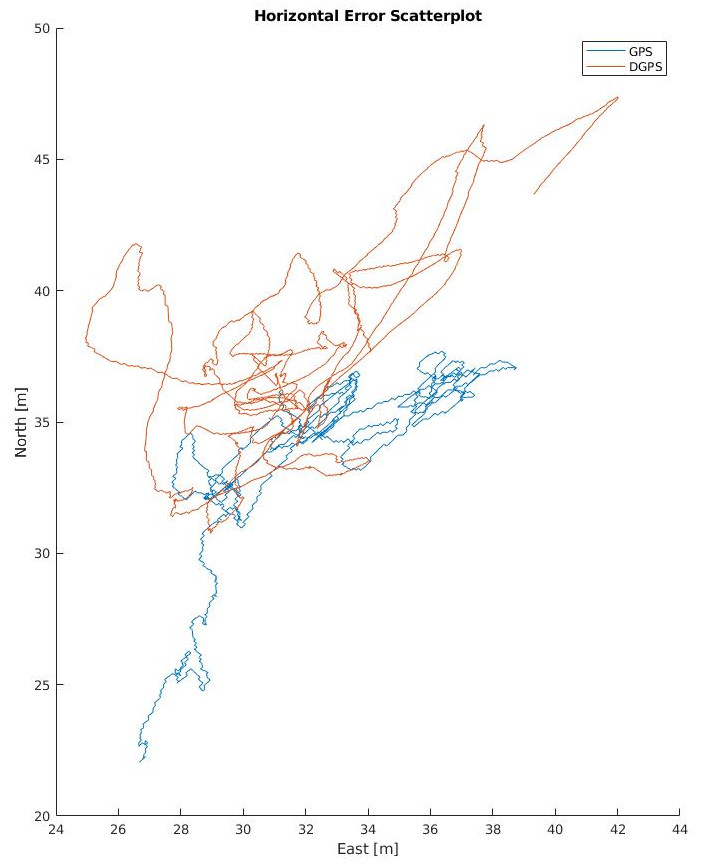
\includegraphics[width=0.5\textwidth]{images/Scatterplot.jpg}
 \captionof{figure}{Scatterplot of the horizontal errors arround the reference position}
 \label{fig:scatterplot}
\end{wrapfigure}

Figure \ref{fig:horizontal_vertical_error} shows the horizontal errors on the left and the vertical errors on the right.
The vertical error of standard GPS is about in the range it could be expected with an RMS error of 11.75 meters.
The horizontal error of standard GPS on the other hand has an RMS error of 45.46 meters.
This is much more than the 10 meter 95th percentile specified in the GPS Performance Stardard.

It is evident that DGPS did not improve those errors distinctly.
Its horizontal error is a bit worse with 49.29 meters RMS and the vertical error a bit better with 8.75 meters RMS than standard GPS.
So there was a small improvement in the vertical error which is the important part of the rocket position for the control.
But it is still far off the 1 meter RMS error defined in the requirements.

Figure \ref{fig:prcs_filtered} shows the PRCs that were calculated by the DGPS Message Generator and applied by the DGPS receiver.
The PRC of 11 GPS satellites were calculated during the test.
About 8 PRCs were available to the DGPS receiver at a time.
They have an average absolute value of 6.8 meters.
The PRC of satellite 2 increaset to -84 meters before is stopped being calculated.
It could be responsible for the increased vertical error of the DGPS solution at arround 1800 seconds.
Such PRCs should be excluded from the RTCM stream in the future.

\begin{figure}[!h]
 \centering
 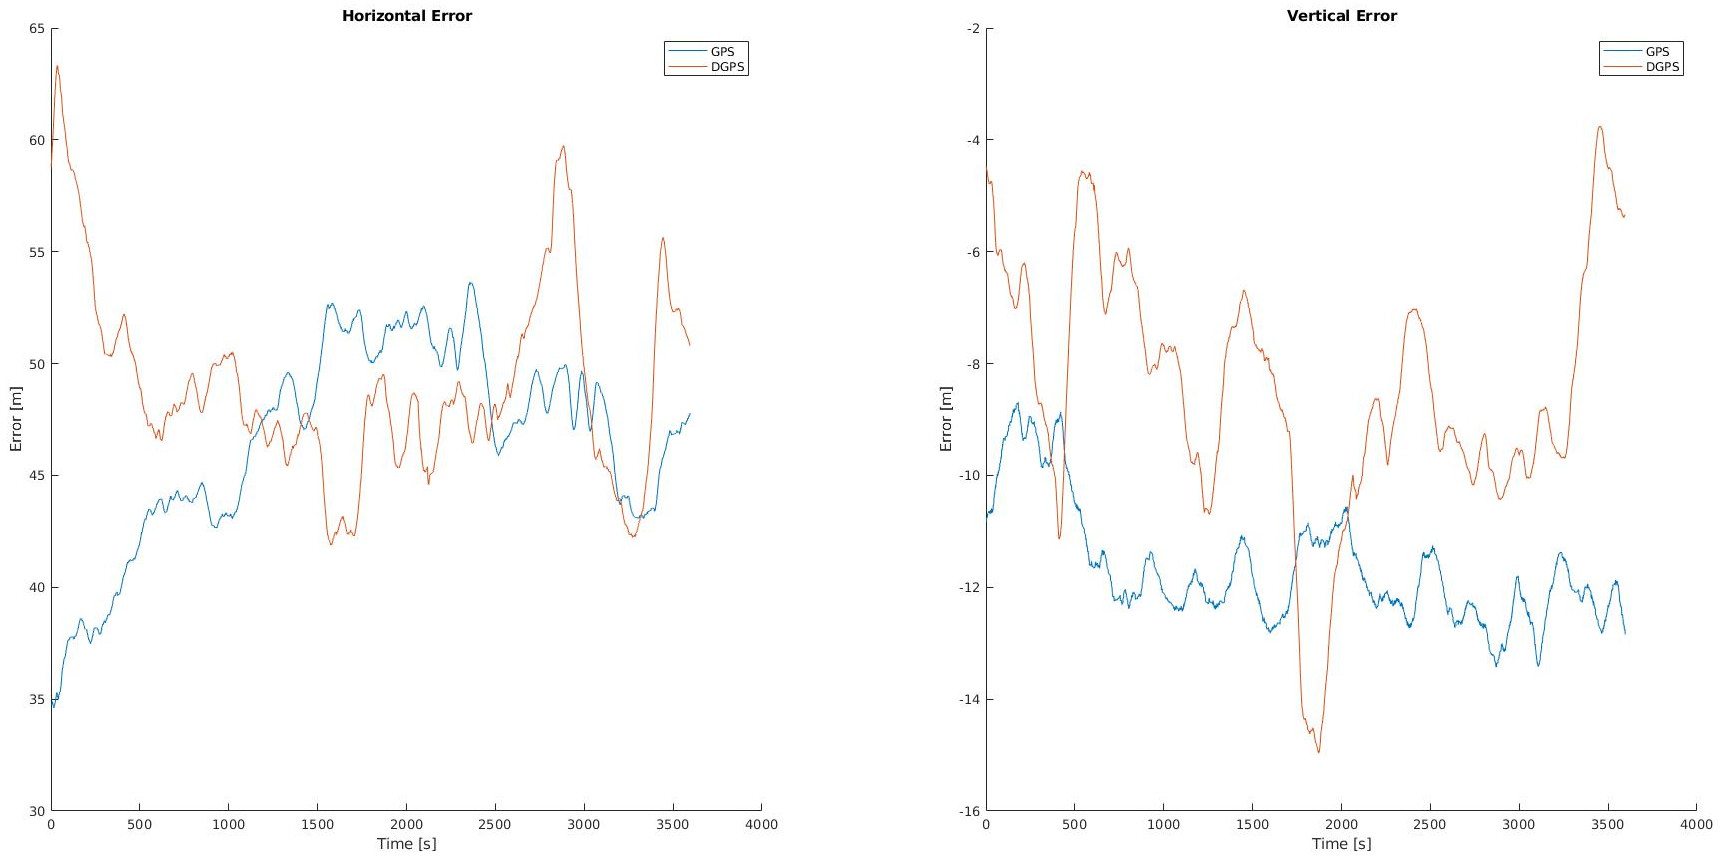
\includegraphics[height=0.4\textheight]{images/Horizontal_Vertical_Error.jpg}
 \caption{Horizontal and vertical errors arround the reference position}
 \label{fig:horizontal_vertical_error}
\end{figure}

\begin{figure}[!h]
 \centering
 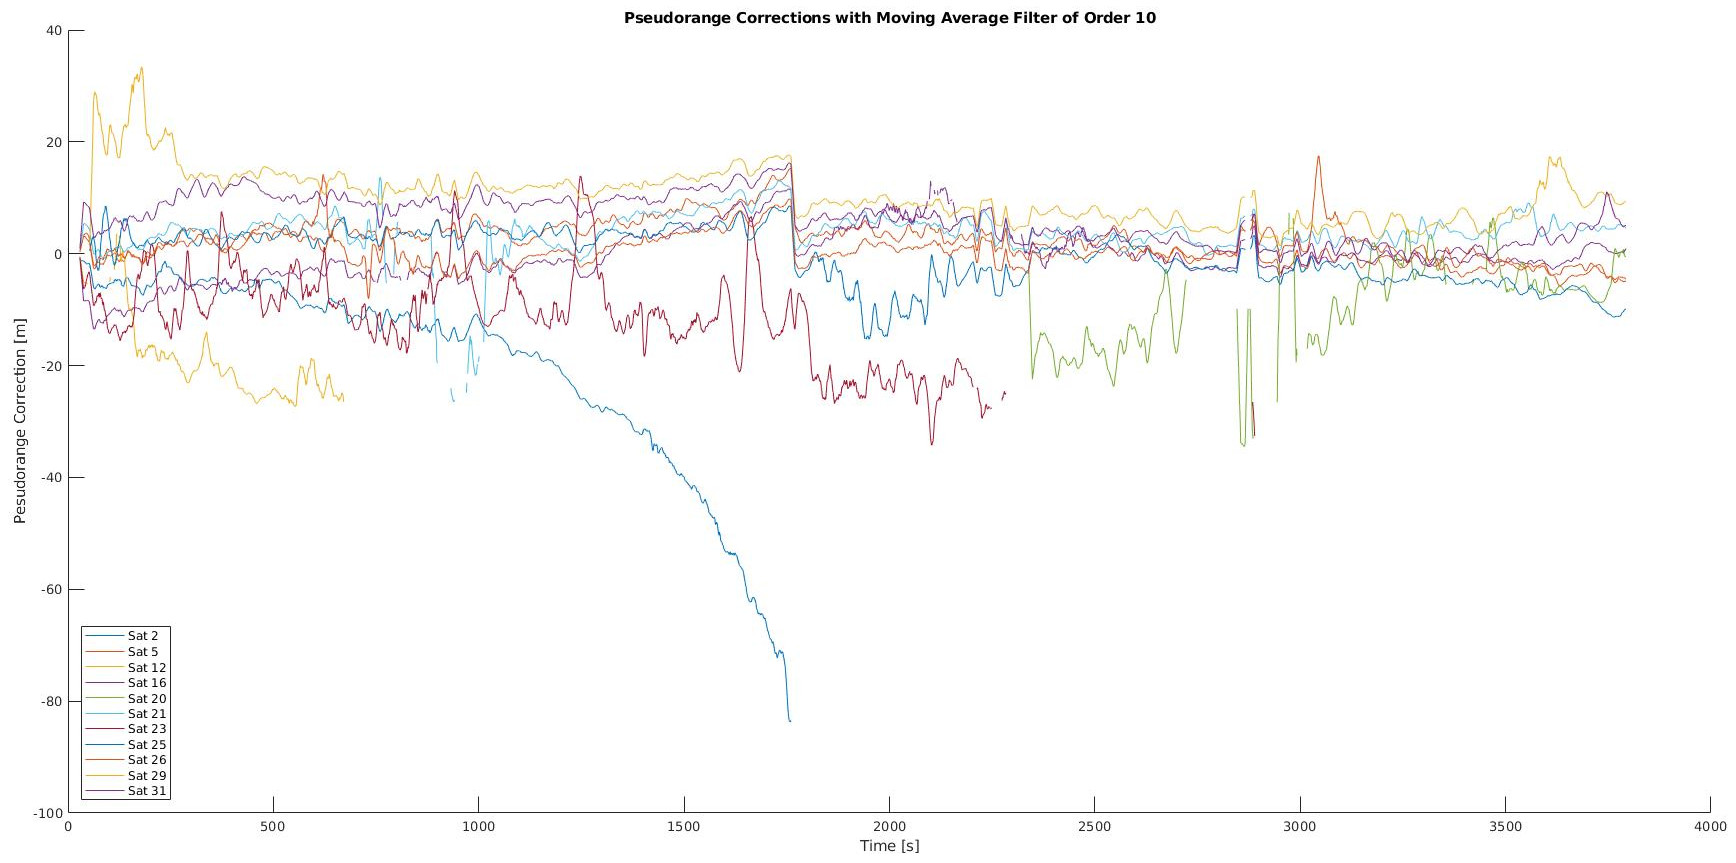
\includegraphics[height=0.4\textheight]{images/PRCs_filtered.jpg}
 \caption{Filtered pseudorange corrections produced by the DGPS Message Generator}
 \label{fig:prcs_filtered}
\end{figure}

\section{Pending Tests}

This secion lists all the tests that were planned but could not be conducted due to time constraints.
Because of the results from the satatic accuracy test, it would also not make sense to test the other scenarios.
The system will probably not produce more accurate results than standard GPS in special conditions when it did not do so in the static test.
The static accuracy would have to be improved first.

\subsection{Mobile Accuracy}

This test is similar to the static accuracy test.
The difference is that the two receivers that estimate the position with and without DGPS corrections move along a pre defined track.
An additional GPS receiver is nedded because the reference receiver can not be used as the standard GPS user anymore.
Also a wireless link is needed to transmit the RTCM stream from the reference station to the user.
The XBee module could be used for this purpose like it was planned for the final implementation.

\subsection{Horizontal Distance}

To measures how well he errors are correlated over a horizontal distance, the reference station and the user will be separated by a distance of about 5 km.
The setup can be the same as in the mobile accuracy test.
The PRCs should still have a positive impact on the position estimation.

\subsection{Height Difference}

A height difference between the reference station and the user can lead to a difference in their tropospheric errors.
If a difference of 3 km has a big impact on the user position accuracy is tested here.
The user receiver is placed on a mountain with a height of about 3 km.
It has a wireless connection to the reference station in the valley.
The range of the XBee module should be sufficient for such a test.
If the height difference has a big impact on the user position accuracy, a differential tropospheric model would have to be added to the PRCs to compensate for it.

\subsection{Telemetry Antenna Interference}

Because the telemetry transmitter on TELL has a transmitting power of 1 W and is placed right next to the GPS antennas, it has to be tested how big its impact on the carrier-to-noise-density ratio is.
With a decrease in the carrier-to-noise-density ratio increases the receiver noise and the position error.
Before it is tested, it should be roughly calculated to make sure the GPS receiver is not damaged.
The test can be done with a standard GPS receiver without DPGS.

\subsection{Antenna Rotation}

Sounding rockets normally rotate to stabilize their trajectory.
A rotation of the GPS antenna can result in a varying signal strenght especially for signals from GPS satellites with low elevations.
It has to be tested how fading affects the GPS receiver.

\subsection{Correction Message Interruption}

During the launch of the rocket, it could come to an interruption of the telemetry link.
This would also interrupt the RTCM stream.
It is tested how long the receiver on the rocket could continue to provide an accurate DGPS position with the old corrections.

\subsection{Rocket Test}

A final validation of the system can only be made with a rocket launch.
Especially if the receiver can handle the acceleration is only possible to test this way.

